\section{Results}
\label{sec:results}
We distinguish historical emitted decisions from the revised implementation and reanalysis. All numerical tables below are generated from the preserved packets or study responses; no historical predictor was retrained.

\subsection{Structured evidence in the exploratory study}
\label{sec:human-results}
Table~\ref{tab:human-study-summary} reports recomputed averages, paired effects and revised statistical tests. Diagnostic and remediation accuracy increase from 0.5625 to 0.921875, a difference of 0.359375. Confidence increases from 3.078125 to 4.234375. These aggregates match the historical data; revised p-values differ because a single bilateral procedure and multiplicity correction replace the previously underspecified tests. Longer evidence statements are descriptive and do not establish better reasoning. The experiment supports a benefit of the complete evidence bundle on these standardized tasks, with the limitations in Section~\ref{sec:human-study}.
\begin{table*}[t]
\centering
\small
\caption{Exploratory N=16 study; 64 case responses per condition. Participant means and paired differences with 95\% participant-bootstrap intervals. $p_H$ is the two-sided signed-rank sign-enumeration p-value adjusted by Holm over four endpoints; diagnosis/remediation correctness coincides in all 128 responses.}
\label{tab:human-study-summary}
\begin{tabular}{lrrrr}
\toprule
Outcome & A & B & Difference [95\% CI] & $p_H$ \\
\midrule
Diagnosis & 0.562 & 0.922 & 0.359 [0.203, 0.516] & 0.00293 \\
Remediation & 0.562 & 0.922 & 0.359 [0.203, 0.516] & 0.00293 \\
Confidence & 3.078 & 4.234 & 1.156 [0.922, 1.375] & 0.00012 \\
Evidence (characters) & 69.812 & 91.656 & 21.844 [20.047, 23.734] & 0.00012 \\
\bottomrule
\end{tabular}
\end{table*}

\begin{table}[t]
\centering
\small
\caption{Diagnostic counts by case and condition. Every cell has eight responses; case materials are standardized research scenarios.}
\label{tab:human-study-keycases}
\begin{tabular}{lrr}
\toprule
Case & A & B \\
\midrule
C1 & 5/8 & 7/8 \\
C2 & 4/8 & 8/8 \\
C3 & 4/8 & 8/8 \\
C4 & 7/8 & 7/8 \\
C5 & 5/8 & 7/8 \\
C6 & 3/8 & 7/8 \\
C7 & 6/8 & 7/8 \\
C8 & 2/8 & 8/8 \\
\bottomrule
\end{tabular}
\end{table}

\begin{figure}[t]
\centering
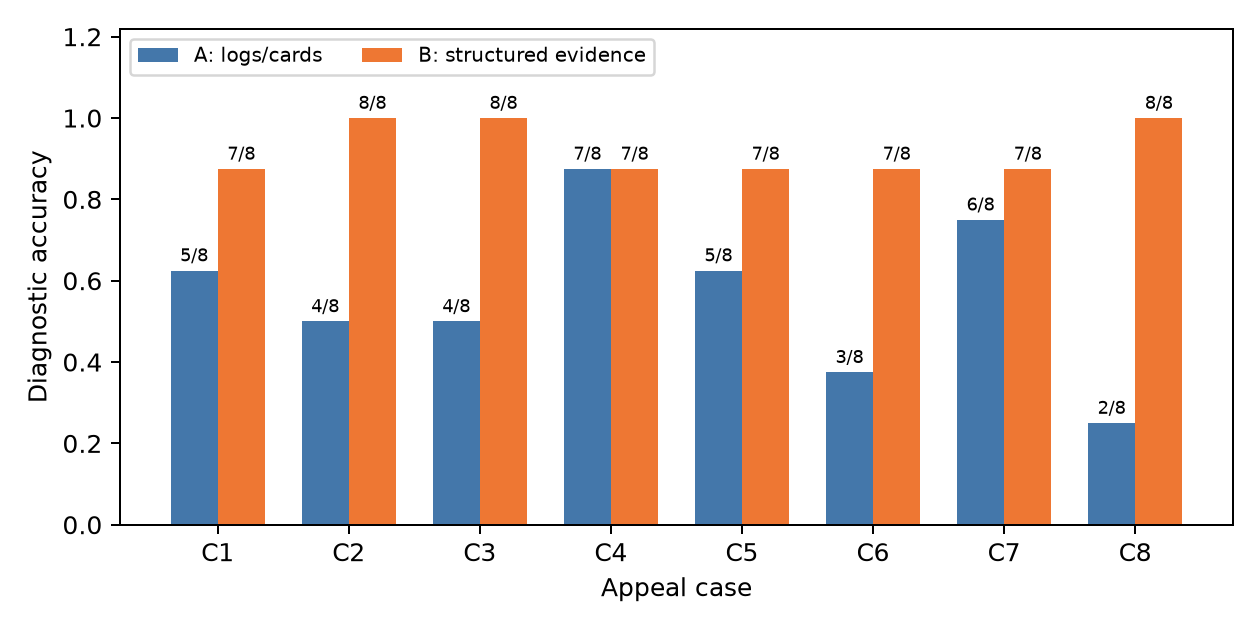
\includegraphics[width=\linewidth]{figures/human_label_accuracy_by_case.png}
\caption{Diagnostic accuracy by case and condition. Labels give exact correct/total counts; all bars have eight responses.}
\Description{Grouped bars compare baseline A and structured-evidence B across eight appeal cases. B equals A in C4 and is higher in the other seven cases. Exact numerators and denominators appear in the adjacent case-count table.}
\label{fig:human-by-case}
\end{figure}

\subsection{Historical states and capacity}
Table~\ref{tab:run-initial} recomputes the historical recipe outcomes and Table~\ref{tab:state-counts} gives exact counts. In the synthetic example $K=100$ but only four cases are eligible and selected; coverage 0.004 is therefore consistent with the capacity ceiling. OULAD similarly selects 69 of a possible 500. Violations were recorded by the historical runner; those records alone do not prove operational escalation.
\begin{table*}[t]
\centering
\small
\caption{PosRate is the selected-set positive outcome rate (legacy Utility@K), not intervention benefit. Historical recipe outcomes, recomputed from emitted states. Entropy thresholds are in bits; VIOL indicates a retrospective ECL violation, not a delivered human review.}
\label{tab:run-initial}
\begin{tabular}{lrrrrrrl}
\toprule
Dataset & $K$ & $\gamma$ & PosRate & Coverage & Abstain & Gap & ECL \\
\midrule
ASSISTments & 1000 & 0.60 & 0.981 & 0.758560 & 0.241440 & 0.00497 & OK \\
OULAD & 500 & 0.60 & 0.174 & 0.010584 & 0.989416 & 0.00192 & VIOL \\
Synthetic & 100 & 0.65 & 1.000 & 0.004000 & 0.996000 & 0.00895 & VIOL \\
\bottomrule
\end{tabular}
\end{table*}

\begin{table*}[t]
\centering
\small
\caption{Exact initial state counts. $K$ is a capacity ceiling, not the realized number selected.}
\label{tab:state-counts}
\begin{tabular}{lrrrrr}
\toprule
Dataset & $n$ & Eligible & Select & Reject & Abstain \\
\midrule
ASSISTments & 105107 & 79730 & 1000 & 78730 & 25377 \\
OULAD & 6519 & 69 & 69 & 0 & 6450 \\
Synthetic & 1000 & 4 & 4 & 0 & 996 \\
\bottomrule
\end{tabular}
\end{table*}


\subsection{Fixed-budget recovery and variable-budget profiles}
Table~\ref{tab:run-sweep} separates full-grid and fixed-budget counts. Table~\ref{tab:recovered} reports achieved metrics of the revised fixed-budget MAS choices. Raising $\gamma$ recovers sample feasibility without retraining, demonstrating a policy-level route to resolve the particular violation. This does not exclude simultaneous model or measurement problems. Table~\ref{tab:policy-profiles} reports separate variable-budget comparisons with the complete profile definitions in Section~\ref{sec:method}. Full precision, group counts, exact grids and candidate IDs are in the structured revision report.
\begin{table}[t]
\centering
\small
\caption{Candidate counts under gap $\leq0.05$ and coverage $\geq0.50$. Full grids vary $K$ and $\gamma$; fixed-budget analyses use only the 16 thresholds at the recipe budget.}
\label{tab:run-sweep}
\begin{tabular}{lrrrrr}
\toprule
Dataset & Full & Feas. & Fixed & Feas. & Pareto \\
\midrule
ASSISTments & 80 & 55 & 16 & 11 & 1 \\
OULAD & 80 & 15 & 16 & 3 & 1 \\
Synthetic & 80 & 12 & 16 & 3 & 1 \\
\bottomrule
\end{tabular}
\end{table}

\begin{table*}[t]
\centering
\small
\caption{Revised MAS selections from the fixed-$K$ feasible Pareto set. All tie tolerances are zero; persistent candidate ID is the final tie-breaker.}
\label{tab:recovered}
\begin{tabular}{lrrrrrrr}
\toprule
Dataset & $K$ & $\gamma$ & Selected & Utility & Gap & Coverage & Abstain \\
\midrule
ASSISTments & 1000 & 0.999 & 1000 & 0.981 & 0.00497 & 0.999448 & 0.000552 \\
OULAD & 500 & 0.999 & 500 & 0.732 & 0.01345 & 0.906427 & 0.093573 \\
Synthetic & 100 & 0.999 & 100 & 1.000 & 0.01697 & 0.933000 & 0.067000 \\
\bottomrule
\end{tabular}
\end{table*}

\begin{table*}[t]
\centering
\small
\caption{Variable-$K$ profiles over the full 80-point grids; these are distinct from fixed-budget recovery. Fairness-first orders gap, utility, abstention; utility-first orders utility, gap, abstention.}
\label{tab:policy-profiles}
\begin{tabular}{llrrrrr}
\toprule
Dataset & Profile & $K$ & $\gamma$ & Utility & Gap & Coverage \\
\midrule
ASSISTments & Fairness-first & 100 & 0.999 & 0.980 & 0.00040 & 0.999448 \\
ASSISTments & Utility-first & 250 & 0.999 & 0.992 & 0.00206 & 0.999448 \\
OULAD & Fairness-first & 50 & 0.999 & 0.800 & 0.00685 & 0.906427 \\
OULAD & Utility-first & 100 & 0.999 & 0.830 & 0.00754 & 0.906427 \\
Synthetic & Fairness-first & 20 & 0.999 & 1.000 & 0.00020 & 0.933000 \\
Synthetic & Utility-first & 20 & 0.999 & 1.000 & 0.00020 & 0.933000 \\
\bottomrule
\end{tabular}
\end{table*}


\subsection{Taxonomy and uncertainty}
Table~\ref{tab:policy-replay} fixes scores, $K$ and $\gamma$ while changing abstention semantics. Utility stays fixed in this example, but automation coverage changes because non-selection can be an automated rejection or a deferral. Treating this as a policy correction requires institutional justification; the numbers alone cannot establish which responsibility assignment is appropriate.
\begin{table*}[t]
\centering
\small
\caption{ASSISTments taxonomy replay with fixed scores, $K=1000$ and $\gamma=0.60$ bits. Changes in automation coverage represent changes in decision responsibility, not demonstrated improvement in student outcomes.}
\label{tab:policy-replay}
\begin{tabular}{lrrrr}
\toprule
Policy & Utility & Coverage & Abstain & Gap \\
\midrule
Global abstention & 0.981 & 0.758560 & 0.241440 & 0.00497 \\
Top-K-only abstention & 0.981 & 1.000000 & 0.000000 & 0.00497 \\
Defer remainder & 0.981 & 0.009514 & 0.990486 & 0.00497 \\
\bottomrule
\end{tabular}
\end{table*}


Table~\ref{tab:uncertainty_proxy_validation} incorporates the previously disconnected numerical validation, recalculated with one entropy convention and average ranks for ties. OULAD has lower entropy/error monotonicity than ASSISTments; the synthetic predictor is poorly calibrated. Temperature scaling can worsen ECE, so we do not claim calibration robustness from preserved rank correlation. The report includes conditional row-bootstrap intervals and group-specific error counts and Wilson intervals across thresholds. Historical interaction packets lack student cluster IDs, so the ASSISTments intervals do not establish cluster-robust uncertainty or field reliability.
\begin{table}[t]
\centering
\small
\caption{Recomputed entropy validation. ECE uses 10 equal-width probability bins including score 1; Spearman uses average ranks for ties. Both baseline and temperature stress use entropy in bits.}
\label{tab:uncertainty_proxy_validation}
\begin{tabular}{lrrrr}
\toprule
Dataset & ECE & $\rho$ & ECE ($T=2$) & $\rho$ ($T=2$) \\
\midrule
ASSISTments & 0.0271 & 0.9789 & 0.0905 & 0.9818 \\
OULAD & 0.0128 & 0.4166 & 0.0703 & 0.4166 \\
Synthetic & 0.2914 & 0.6774 & 0.2398 & 0.6774 \\
\bottomrule
\end{tabular}
\end{table}


\subsection{Artifact checks and appeal scope}
The historical four-point scorecard was populated by constant booleans in the runner, so it is not evidence of independent artifact validation. The revised verifier instead computes integrity and decision-reconstruction checks and tests failures after packet tampering or missing policy content. Fitted-model hashes are separated from configuration hashes; the earlier configuration-only digest is not presented as an immutable trained-model identity.

The appeal pack (Table~\ref{tab:appeal_scenarios}) is a set of study materials. Medical exceptions, changing income, or removing a feature require additional policy inputs or re-scoring and are outside the fixed-score replay contract. Evidence strings in these materials are not execution logs proving that the released engine implements those operations.
\begin{table*}[t]
\centering\small
\caption{Illustrative N=16 study materials, not execution logs. Full Portuguese narratives and A/B evidence strings remain in the eight local case JSONs. The scope column distinguishes fixed-score replay from operations that the engine does not implement.}
\label{tab:appeal_scenarios}
\begin{tabularx}{\textwidth}{lp{.18\textwidth}Xp{.24\textwidth}}
\toprule
Case & Diagnostic category & Evidence illustrated in the instrument & Engine scope \\
\midrule
C1 & Stale input data & Income snapshot and update lineage & Corrected inputs require new inference. \\
C2 & Policy change & Policy versions and effective dates & Fixed-score replay only for supported policy fields. \\
C3 & Normative exception & Medical flag and force-inclusion rule & Exception rule and medical inputs are not implemented. \\
C4 & Capacity constraint & School capacity and revised availability & Global K replay supported; per-school capacity is outside the engine. \\
C5 & Fairness constraint & Group gap and policy cap & Retrospective candidate check; no per-person fairness reranking. \\
C6 & Proxy risk & ZIP-code correlation and feature removal & Proxy audit/removal requires additional analysis or fitting. \\
C7 & Abstention error & Uncertainty value and threshold & Supported score-based abstention reconstruction. \\
C8 & Version mismatch & Declared and executed policy hashes & Content/hash consistency check; no CI/CD system integration. \\
\bottomrule
\end{tabularx}
\end{table*}

